% meta.concepts: math; 2D vector
% meta.tags: word problem
% acknowledge: Engineering Statics: Open and Interactive
% source: Example 2.6.4 of January 10, 2023 edition

Vector ${\bf A} = 200 N \angle 45^\circ$ counterclockwise from the $x$ axis, and vector ${\bf B} = 300 N \angle 70^\circ$ counterclockwise from the $y$ axis.

Draw the vectors and find the resultant ${\bf R} = {\bf A} + {\bf B}$ by addition of scalar components.

\vspace{.5cm}
\rule{\textwidth}{.4pt}
\vspace{.5cm}
\textbf{Solution:}
\begin{figure}[ht!]
  \centering
  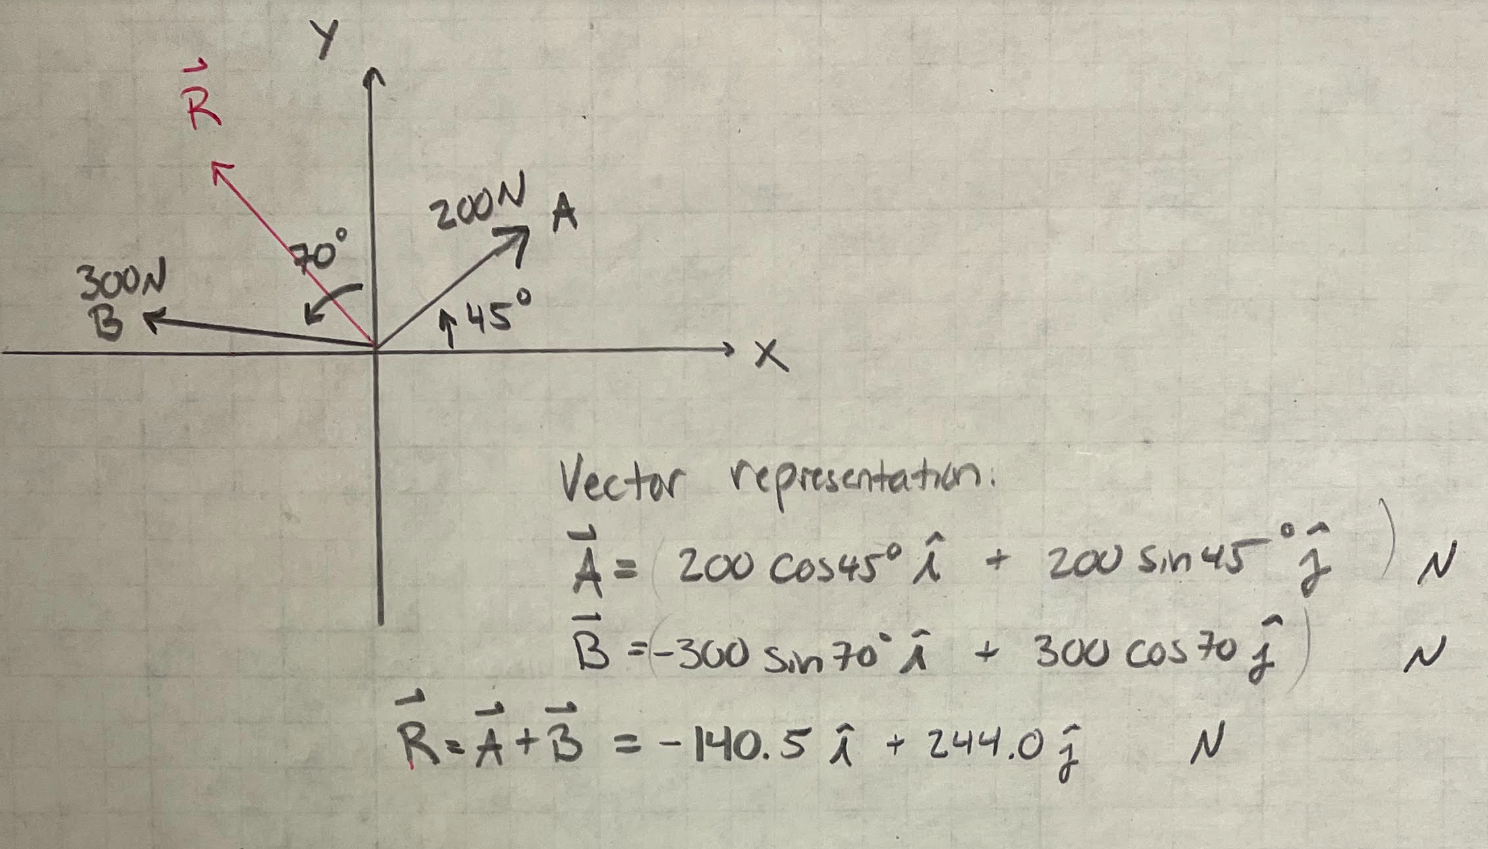
\includegraphics[width=0.9\textwidth]{soln.png}
\end{figure}

%
% Answer
%
% ${\bf R} = 281.6 N \angle 119.9^\circ$ counterclockwise from the $x$ axis.
